\documentclass[11pt, letterpaper]{article}
\usepackage{graphicx} % Required for inserting images
\usepackage{fancyhdr}
\usepackage{amsmath}
\usepackage{tcolorbox}
\usepackage{authblk}
\usepackage{indentfirst}
\usepackage{geometry}
\geometry{left=3cm,right=3cm,top=3cm,bottom=3cm}
\graphicspath{ {./images/} }

\fancypagestyle{plain}{
  \fancyhead[L]{Design Patterns}
  \fancyhead[R]{EasyCollab}
  \renewcommand{\headrulewidth}{0.4pt}
  \renewcommand{\footrulewidth}{0.4pt}
}

\title{Projet de Design Patterns}
\author{EasyCollab\\Aboubacar HASSANE CHEKOU KORE, Théo JOFFROY, Louis LESNIAK}
\date{31 Décembre 2023}

\begin{document}

\maketitle

\section{Rapport}
\subsection{Fonctionnalités réalisées}

\begin{itemize}
\item \textbf{Création d'un compte}

Formulaire accessible depuis le bouton "Créer un compte" sur la page d'accueil

\item \textbf{Connexion à un compte existant}

Formulaire accessible depuis le bouton "Se connecter" sur la page d'accueil

\item \textbf{Création d'un document vide}

Depuis le bouton "Créer un document" sur la page d'accueil, l'utilisateur doit préciser le nom du document.

\item \textbf{Ouverture d'un document sauvegardé}

Les documents créés par l'utilisateur apparaissent sur la page d'accueil lorsqu'il est connecté. Pour en ouvrir un, il suffit de cliquer sur son nom.

\item \textbf{Modification d'un document}

Une fois un document ouvert, il suffit de changer le contenu des cellules pour modifier le document.
Il est aussi possible de changer le nom d'un document en cliquant sur le bouton "Renommer" qui lui est associé depuis la page d'accueil.


\item \textbf{Sauvegarde d'un document}

La sauvegarde des modifications est réalisée automatiquement à chaque saisie de caractère dans une cellule.
Le changement de nom d'un document est sauvegardé lors de la validation.

\item \textbf{Suppression d'un document}

Possible en cliquant sur le bouton "Supprimer" associé au document depuis la page d'accueil.

\item \textbf{Persistance des données}

Toutes les données (utilisateurs et documents) sont sauvegardées dans un fichier côté serveur.

\item \textbf{Partage d'un document sauvegardé avec d'autres utilisateurs}

Il est possible de partager un document que l'on a soi-même créé à un autre utilisateur en saisissant son nom dans le champ associé à chaque document depuis la page d'accueil. On ne peut partager le document ni à soi-même ni à un utilisateur non inscrit. Les utilisateurs à qui l'on a partagé un document peuvent l'ouvrir (depuis la page d'accueil une fois qu'ils sont connectés), le modifier et ces modifications sauvegardées.
Seul l'utilisateur qui a créé le document peut le supprimer.

\item \textbf{Affichage des utilisateurs travaillant simultanément sur le même document}

Tous les noms des utilisateurs ayant ouvert un même document simultanément sont visibles au-dessus du tableur.

\item \textbf{Mise à jour en temps réel de l'affichage}

Les modifications d'un utilisateur sont visibles instantanément pour tous les autres utilisateurs ayant ouvert le document.
\end{itemize}

\subsection{Conception et difficultés rencontrées}

Pour la partie inscription/connexion, nous nous sommes très largement inspiré du modèle vu en cours, ce qui a accéléré le développement. La persistance des données est réalisée grâce à un fichier au format $JSON$, l'interface avec ce format étant très simple d'utilisation en $Javascript$. Le temps réel est pris en charge grâce à la technique du $long$ $polling$.

\begin{figure}[htp]
    \centering
    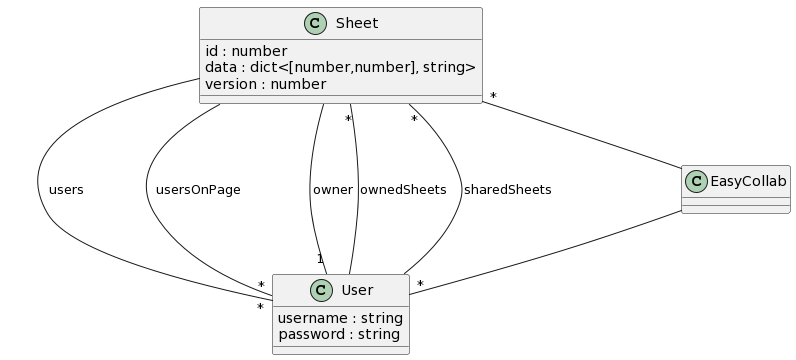
\includegraphics[width=14cm]{images/class_diagram.png}
    \caption{Diagramme de classes de l'application}.
\end{figure}

La version présentée lors du point de suivi nécessitait de transmettre l'intégralité du document dans la requête effectuant la sauvegarde (seules les cellules vides n'étaient pas transmises). Il était difficilement envisgeable de conserver un processus aussi lourd dans le cas où un document était volumineux, nous sommes donc parvenus à faire en sorte que seule la cellule modifiée soit transmise dans la requête (un listener est attaché à l'event $keyup$ de chaque cellule et il déclenche l'envoi d'une requête paramétrée avec un objet contenant les coordonnées de la cellule ainsi que son contenu).

\subsection{Déroulé du projet}

Concernant la répartition du travail, Théo s'est occupé de la réalisation des fonctionnalités de base (Inscription, connexion, création d'un document, modification, sauvegarde et suppression), Louis s'est chargé du partage des documents entre les utilisateurs et de l'aspect temps réel et Aboubacar a travaillé sur le front-end de l'application.

\newpage
\section{Documentation}

\subsection{Guide d'installation}

Spécifiez dans le fichier $.env$ (ou $.env.local$) les champs
\verb+SECRET+ et \verb+PORT+.
Le port par défaut est le port $3000$, vous pouvez générer 64 bytes aléatoirement pour spécifier le champ \verb+SECRET+ à l’aide de la commande javascript :
\begin{verbatim}
    require('crypto').randomBytes(64).toString('hex’)
\end{verbatim}
Ensuite, entrez dans votre terminal :
\begin{verbatim}
    npm install && npm start
\end{verbatim}

\subsection{Connexion au serveur}

Ouvrir la page : \verb+http://localhost:PORT+

(où \verb+PORT+ est le port défini dans le fichier $.env$ (ou $.env.local$), si vous n’avez pas défini de port, il est de $3000$ par défaut.)

\subsection{Description des routes}

Il y a cinq méthodes de requêtes sur $EasyCollab$ : \verb+GET+, \verb+POST+, \verb+PUT+, \verb+PATCH+ et \verb+DELETE+. Nous allons vous détailler l’intégralité des routes pour chacune de ces méthodes.

\subsubsection*{\textbf{GET}} 
\begin{itemize}
    \item \verb+/+
    
    Affichage de la page d’accueil du site.
    \begin{itemize}
        \item Si l’utilisateur n’est pas connecté, il y verra une description du site et deux boutons : "Se connecter" et "Créer un compte". 
        \item  S'il est connecté, il y verra la page de gestion de ses documents et les documents qu’il lui ont été partagés.
    \end{itemize}

    \item \verb+/account/signin+
    
    Formulaire de connexion au site (utilisateur et mot de passe).
    
    \item \verb+/account/signup+
    
    Formulaire d’inscription au site (utilisateur, mot de passe et confirmation du mot de passe).

    \item \verb+/account/signoff+
    
    Permet à l’utilisateur de se déconnecter.

    \item \verb+/sheet/new+
    
    Formulaire de création d’un nouveau document (nom du document).

    \item \verb+/sheet/:sheetId+
    
    Consultation d’un document avec l’identifiant \verb+sheetId+.

    \item \verb+/sheet/update/:sheetId+

    Non accessible par l’utilisateur, elle existe pour une raison technique ($long$ $polling$). Cette route permet de recevoir les données du document partagé d’identifiant \verb+sheetId+ lorsque celui-ci a été modifié par un autre utilisateur.

    \item \verb+/sheet/usersOnPage/:sheetId+

    Non accessible par l’utilisateur, elle existe une pour raison technique. Cette route permet à l’utilisateur de recevoir la liste des clients présents sur le document d’identifiant \verb+sheetId+.
    
\end{itemize}

\subsubsection*{\textbf{POST}} 
\begin{itemize}
    \item \verb+/account/signin+

    Permet au serveur de traiter la requête de connexion lorsqu’on valide le formulaire (contient l’identifiant et le mot de passe hashé).

    \item \verb+/account/signup+

    Permet au serveur de traiter la requête d’inscription lorsqu’on valide le formulaire (contient l’identifiant et le mot de passe hashé).

    \item \verb+/sheet/new+

    Permet au serveur de traiter la requête de création de document lorsqu’on valide le formulaire (contient le nom du document à créer).

    \item \verb+/sheet/subscribe/:sheetId+

    Permet à l’utilisateur d’envoyer au serveur qu’il est entrain de consulter le document d’identifiant \verb+sheetId+.

    \item \verb+/sheet/unsubscribe/:sheetId+

    Permet à l’utilisateur d’envoyer au serveur qu’il a fini de consulter le document d’identifiant \verb+sheetId+.

\end{itemize}

\subsubsection*{\textbf{PUT}} 
\begin{itemize}
    \item \verb+/sheet/rename/:sheetId+

    Permet à l’utilisateur d’envoyer au serveur le caractère qu’il vient de taper dans le document d’identifiant \verb+sheetId+ (contient le caractère en question).

\end{itemize}

\subsubsection*{\textbf{PATCH}} 
\begin{itemize}
    \item \verb+/sheet/:sheetId+

    Permet à l’utilisateur d’envoyer au serveur le nouveau nom du document d’identifiant \verb+sheetId+ (contient le nouveau nom du document).
    
    \item \verb+/sheet/users/:sheetId+

    Permet à l’utilisateur d’ajouter un utilisateur pouvant consulter et modifier son document d’identifiant \verb+sheetId+ (contient le nom d’utilisateur de la personne à ajouter).

\end{itemize}

\subsubsection*{\textbf{DELETE}} 
\begin{itemize}
    \item \verb+/sheet/:sheetId+

    Permet à l’utilisateur de retirer un utilisateur pouvant consulter et modifier son document d’identifiant \verb+sheetId+ (contient le nom d’utilisateur de la personne à retirer).

\end{itemize}

\end{document}

